\documentclass{beamer}

\usetheme[progressbar=frametitle]{metropolis}
\setbeamertemplate{frame numbering}[fraction]
\useoutertheme{metropolis}
\useinnertheme{metropolis}
\usefonttheme{metropolis}
\usecolortheme{spruce}
\setbeamercolor{background canvas}{bg=white}
\usepackage{multicol}
\usepackage{amsmath}  %math staff
\usepackage{graphicx}  %import images
\usepackage{float} %control float positions

\title{A Joint Model for Survival and Longitudinal Data Using Shape Invariant Models}
\author{Jinxi Liu}
\begin{document}
	\metroset{block=fill}
	
\begin{frame}
	
	\titlepage
	
\end{frame}


\begin{frame}[t]{Introduction}\vspace{10pt}
Joint models are increasingly used because they provide more efficient estimates and characterize the relationship between longitudinal process and time to event.

Shape invariant model was shown to fit well for analysis of growth data. The advantage of this method is that the parameter estimates for the model have  simple biological interpretations [1].

\end{frame}

\begin{frame}[t]{Shape invariant models}\vspace{10pt}
Beath [1] developed a shape invariant model for infant growth. In the model, a single function is transformed by shifting and scaling to fit each subject.

The basis of the model is that a population has a common characteristic curve or function, which by shifting and scaling can be made to have the form of any individual curve.
\end{frame}

\begin{frame}[t]{Shape invariant models}\vspace{10pt}
\begin{figure}[h!]
	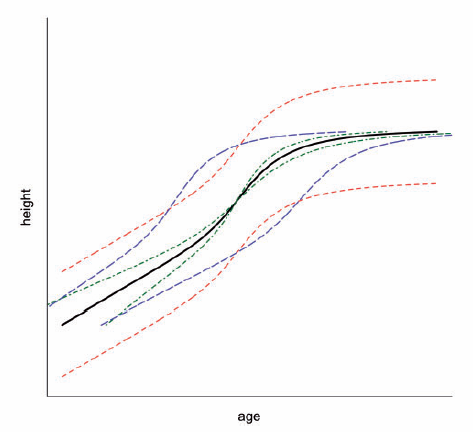
\includegraphics[scale=0.5]{sim.png}
	\caption{Illustration of the SIM for height in puberty. The black solid line is the mean growth curve;the red short dashed lines indicate a vertical or height shift in the curve; the blue long dashed lines indicates a horizontal or age shift and the green dot-dashed lines represent a shrinking/stretching of the age scale}
	\label{fig:sim}
\end{figure}
\end{frame}


\begin{frame}[t]{Shape invariant models}\vspace{10pt}

\begin{equation}
f(\alpha_{0i},\alpha_{1i}, \beta_{0i},\beta_{1i};t) = \alpha_{0i}+e^{\alpha_{1i}}g(\frac{t-\beta_{0i}}{e^{\beta_{1i}}})
\end{equation}
Where $g(t)$ represents the common shape function of the curve and $\alpha_{0i},\alpha_{1i}$ are the shift parameters for the $x$- and $y$-axis, respectively, and $\beta_{0i},\beta_{1i}$ are the corresponding scale parameters.

The function $g(t)$ may either be a parametric or non-parametric function. Beath used a cubic spline. The coefficients of the spline function were treated as fixed effects, resulting in a single spline function for all subjects; and the location and scale parameters ($\alpha_{0i},\alpha_{1i}, \beta_{0i},\beta_{1i}$) as random effects.

\end{frame}

\begin{frame}[t]{Shape invariant models}\vspace{10pt}
Beath demonstrated that the shape invariant model was a useful model for infant growth data. One important feature of the model is that the location and scale parameters have  simple biological interpretation (e.g. in growth curve data, $\alpha_{0i}$ is the size of the infant at the time origin, $\beta_{0i}$ allows for variation of the birth date with respect to the growth curve and $\beta_{1i}$ determines the growth rate).

It would be more useful if we could relate the curve to previous current
exposures and later outcomes.
\end{frame}

\begin{frame}[t]{Joint modeling of time-to-event and repeated measures}\vspace{10pt}
A random changepoint model for joint modeling of cognitive decline and risk of dementia was proposed [2].

The model combines a piecewise polynomial mixed model with a random changepoint for the evolution of the cognitive test and a log-normal model depending on the
random changepoint for the time to dementia.
\end{frame}

\begin{frame}[t]{Joint modeling of time-to-event and repeated measures}\vspace{10pt}
\begin{figure}[h!]
	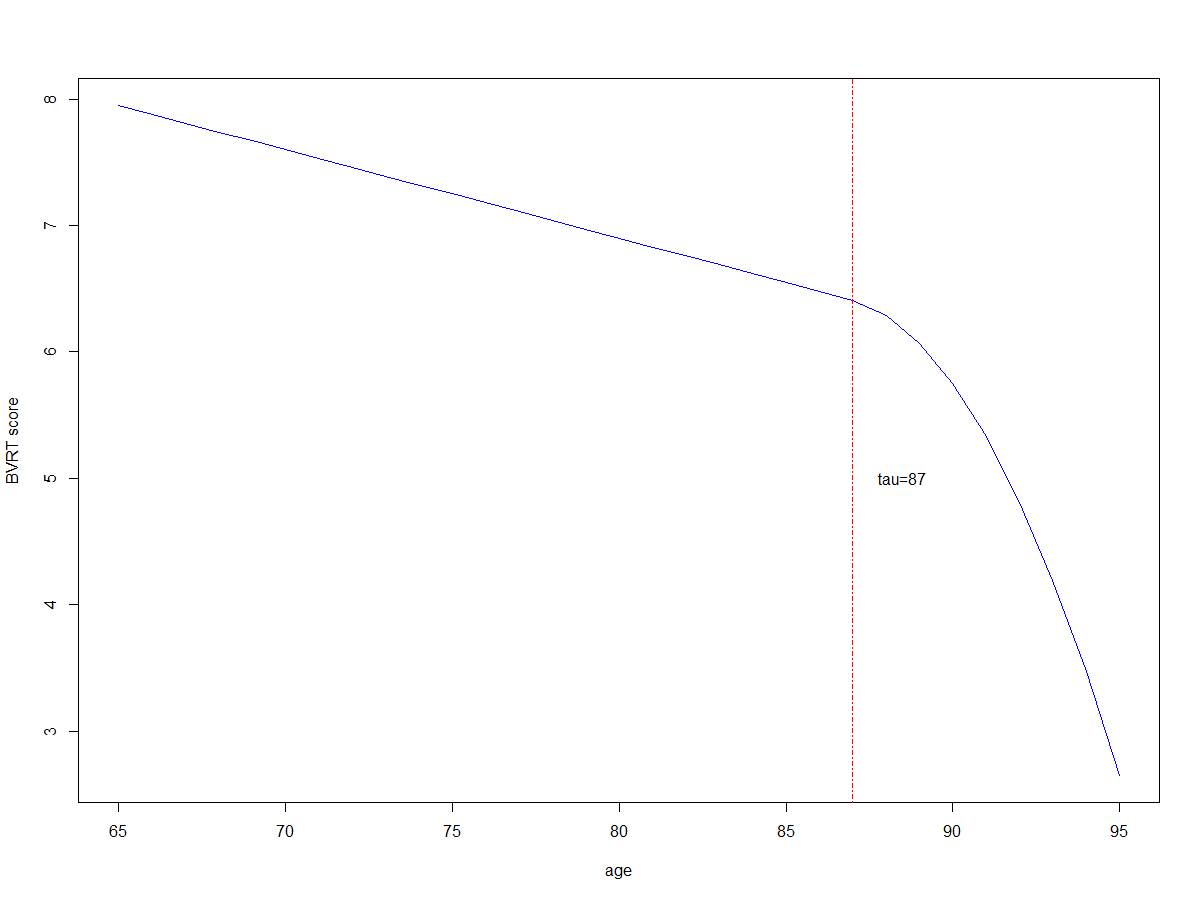
\includegraphics[scale=0.55]{rcp.png}
	\caption{Example of random change point model}
	\label{fig:fig2}
\end{figure}
\end{frame}

\begin{frame}[t]{Joint modeling of time-to-event and repeated measures}\vspace{10pt}
Let $Y_{ij}$ the cognitive test score of subject $i$ at measurement $j$. They assumed a segmented mixed model for $Y_{ij}$ with a linear trend before the changepoint $\tau_{i}$ and a polynomial trend thereafter. The model for cognitive test score is:
\begin{equation}
Y_{ij}=(\mu_0+\mu_{0i})+(\mu_1+\mu_{1i}) \times t_{ij}+\sum_{k=2}^{K}(\mu_k+\mu_{ki}) \times \{(t_{ij}-\tau_i)^{+}\}^k+\epsilon_{ij}
\end{equation}
\begin{figure}[h!]
	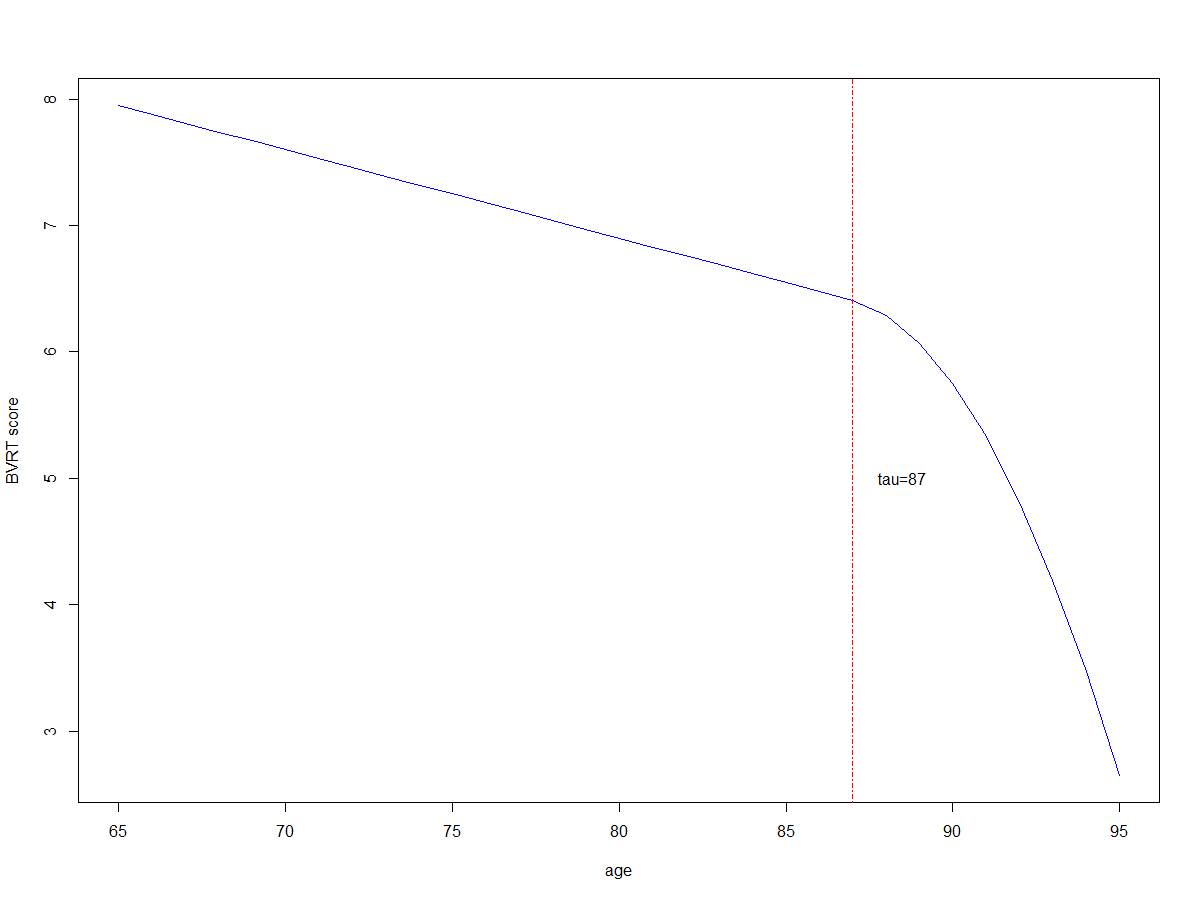
\includegraphics[scale=0.3]{rcp.png}

	\label{fig:fig2s}
\end{figure}
\end{frame}

\begin{frame}[t]{Joint modeling of time-to-event and repeated measures}\vspace{10pt}
Let $X_i = log(T_i)$ the logarithm of age at dementia for subject $i$ and $Z_{xi}$ a row vector of covariates. The random change point $\tau_i$ is assumed to have a lognormal
distribution. The model for age at dementia is:
\begin{equation}
X_i = log(T_i) = Z_{xi}\gamma+\eta log(\tau_i)+\epsilon_{i}
\end{equation}
Parameters were estimated by maximum likelihood. The mean curve for the evolution of the cognitive test or the survival function for the age at dementia given $\tau_i$ can then be computed.

\end{frame}



\begin{frame}[t]{Proposed Model}\vspace{10pt}
We propose a joint model for survival and longitudinal data using the shape invariant models. Our model has two parts, time to event part and longitudinal part.

\end{frame}

\begin{frame}[t]{Proposed Model}\vspace{10pt}
Step 1: Longitudinal component

\begin{equation}
y_{ij}=\alpha_{0i}+e^{\alpha_{1i}}g(\frac{t_{ij}-\beta_{0i}}{e^{\beta_{1i}}}),
\end{equation}
where $y_{ij}$ is the longitudinal outcome of subject $i$ at time $j$, $\alpha_{0i},\alpha_{1i}, \beta_{0i}$ and $\beta_{1i}$ are random effects and $g(\cdot)$ is the common function for mean curve. 

Step 2: Survival component:
\begin{equation}
h_i(t) = h_0(t) \times (exp\{\gamma_1\alpha_{0i}+\gamma_2\alpha_{0i}+\gamma_3\beta_{0i}+\gamma_4\beta_{1i}\})
\end{equation}
\end{frame}

\begin{frame}[t]{Proposed Model}\vspace{10pt}
Step 3: Joint model
\begin{equation}
\begin{split}
L&(Y,T,\delta ; \theta) = \\
&\prod_{i=1}^{N}\int \left\{\prod_{j=1}^{n_i}f(y_{ij}|b_i)\right\} \left\{ h(T_i|b_i) ^{\delta_i} S(T_i|b_i)^{1-\delta_i}\right\} f(b_i) db_i,
\end{split}
\end{equation}
where $T$ is the observed event time, $Y$ is the longitudinal outcome, $\delta$ is event indicator, $\theta$ denotes all parameters in (4) and (5), $b_i$ denoted random effects in (5) (i.e., $\alpha_0,\alpha_1, \beta_0, \beta_1$). $S(\cdot)$ is the survival function and $h(\cdot)$ is the hazard function.

Key assumption:conditional independence of $Y_i$ and $T_i$ given $b_i$.
\end{frame}

\begin{frame}[t]{Application}\vspace{10pt}
Shape invariant model has been proved useful in infant growth data. \\
It might be interesting to test this model on diabetes data. \\
Use HbA1c as longitudinal outcome and cardiovascular event as survival outcome. 

\end{frame}

\begin{frame}[t]{Possible extension}\vspace{10pt}
1. Incorporate time independent/dependent covariates into the model.\\
2. Fit different mean curves for each sub group (treatment arm) separately.\\
3. Multiple longitudinal outcomes.\\
3. Use logistic regression (or other models) instead of survival model. 

\end{frame}

\begin{frame}[t]{Reference}\vspace{10pt}
1. Beath, Ken J. "Infant growth modelling using a shape invariant model with random effects." Statistics in medicine 26.12 (2007): 2547-2564.

2. Jacqmin‐Gadda, Hélène, Daniel Commenges, and Jean‐François Dartigues. "Random changepoint model for joint modeling of cognitive decline and dementia." Biometrics 62.1 (2006): 254-260.
\end{frame}
\end{document}